\chapter{Assembly}

\section{Power and reset}

\subsection{Circuit description}

The figure \ref{fig:artemisa-schematic-power} shows the schematic diagram of the power management and power-on reset circuits.

\begin{figure}[h]
  \centering
  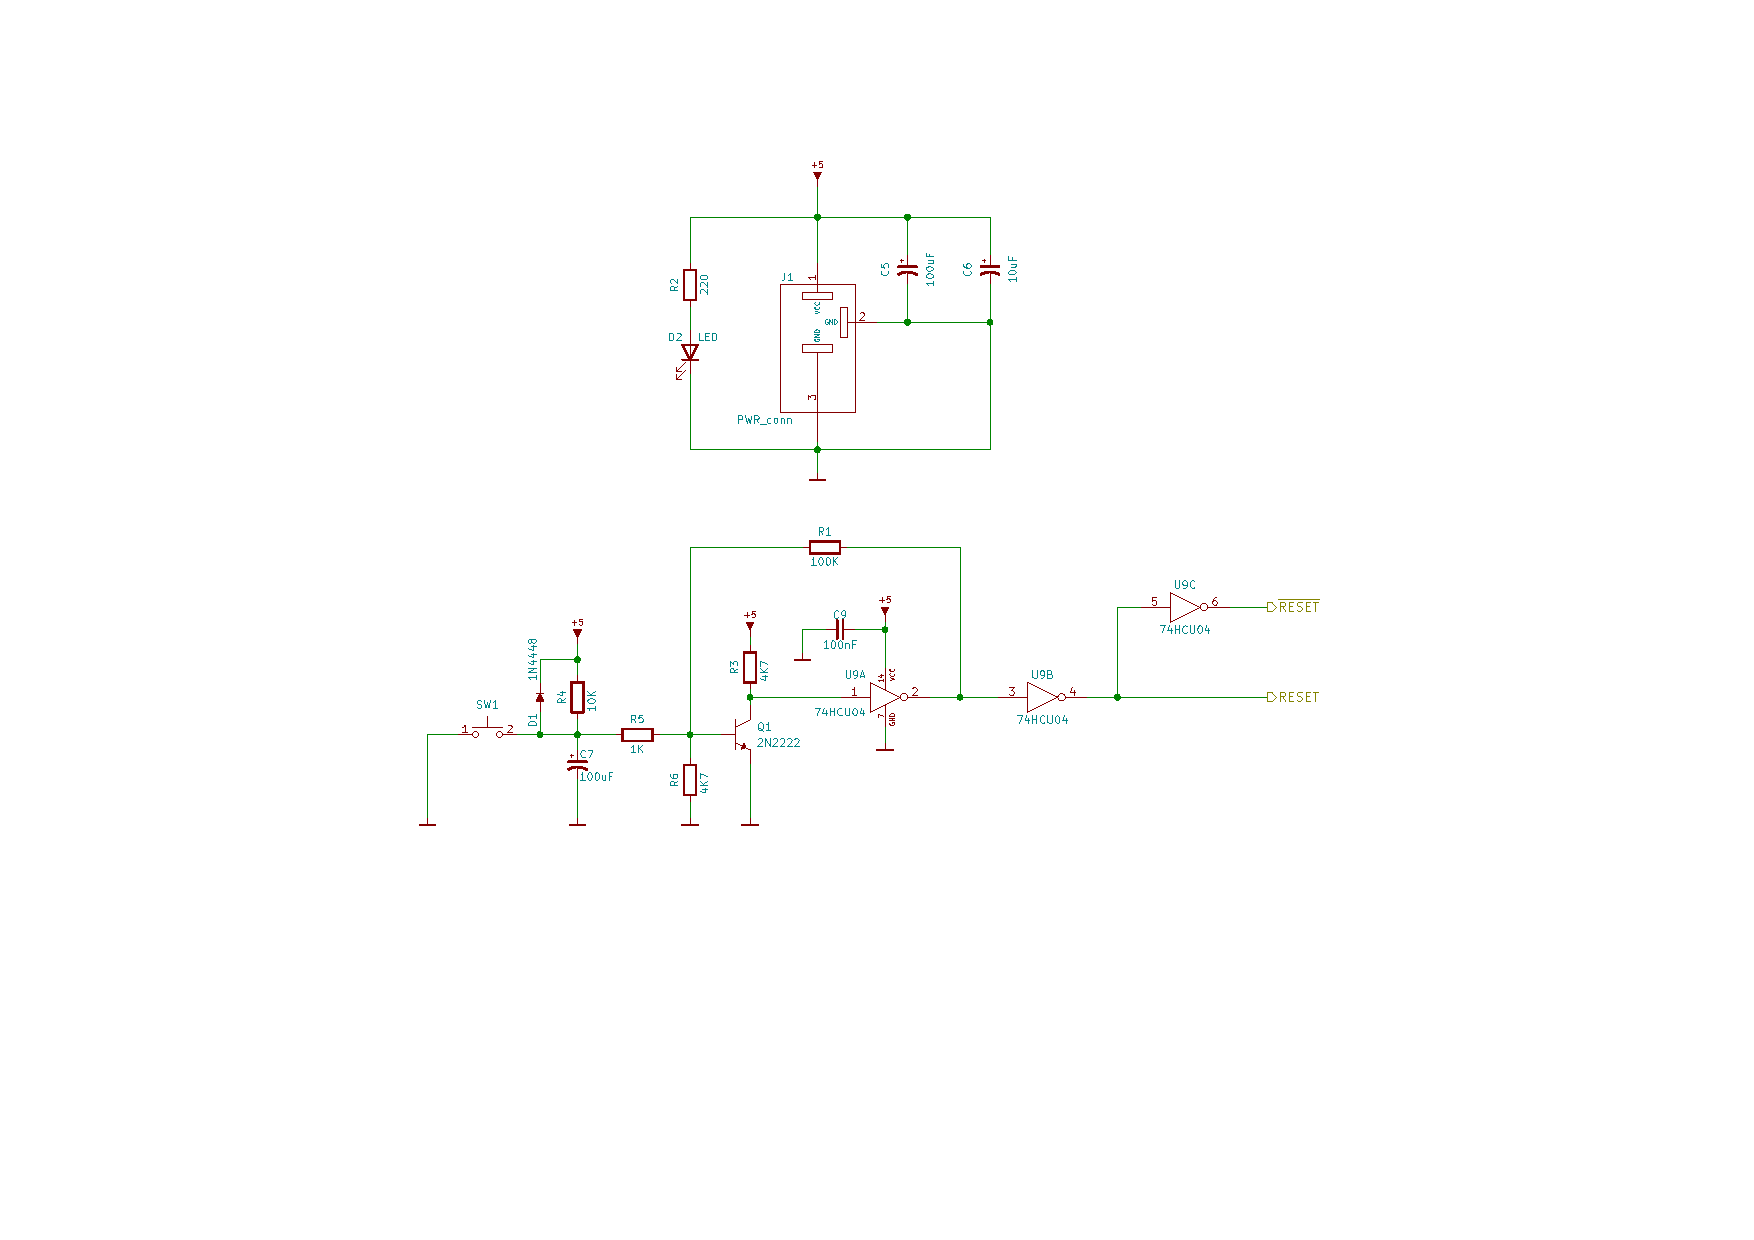
\includegraphics[width=\linewidth,trim={6cm 7cm 6cm 2.5cm},clip]{figures/artemisa-schematic-power}
  \caption{Schematic diagram of power input and power-on reset}
  \label{fig:artemisa-schematic-power}
\end{figure}

As you can see, the schematic sheet is divided in two separated blocks.

\begin{itemize}
  \item At the top side of the schematic we have the power connector circuit. This shows the circuit formed by the DC power barrel connector and a few auxiliary elements around it.
  \item At the bottom side of the schematic we have the power-on reset circuit. This contains the reset button and several components aimed to generate a reset signal to get several computer devices to their initial state.
\end{itemize}

Starting with the power connector. This is extremely simple, as shown in \ref{fig:artemisa-schematic-power-conn}. The DC barrel connector {\tt J1} provides three different terminals: 1, 2 and 3. 1 is the positive input terminal, or {\tt VCC}. 2 and 3 are the negative input terminals, or {\tt GND}. As you can see, they are directly connected to the {\tt +5} and {\tt GND} power symbols, respectively. This means the DC barrel connector is feeding the five volts and the ground inputs. Whenever we see the {\tt +5} and {\tt GND} power symbols in the schematic, we know they are wired to and powered from the {\tt J1} connector.

\begin{figure}[h]
  \centering
  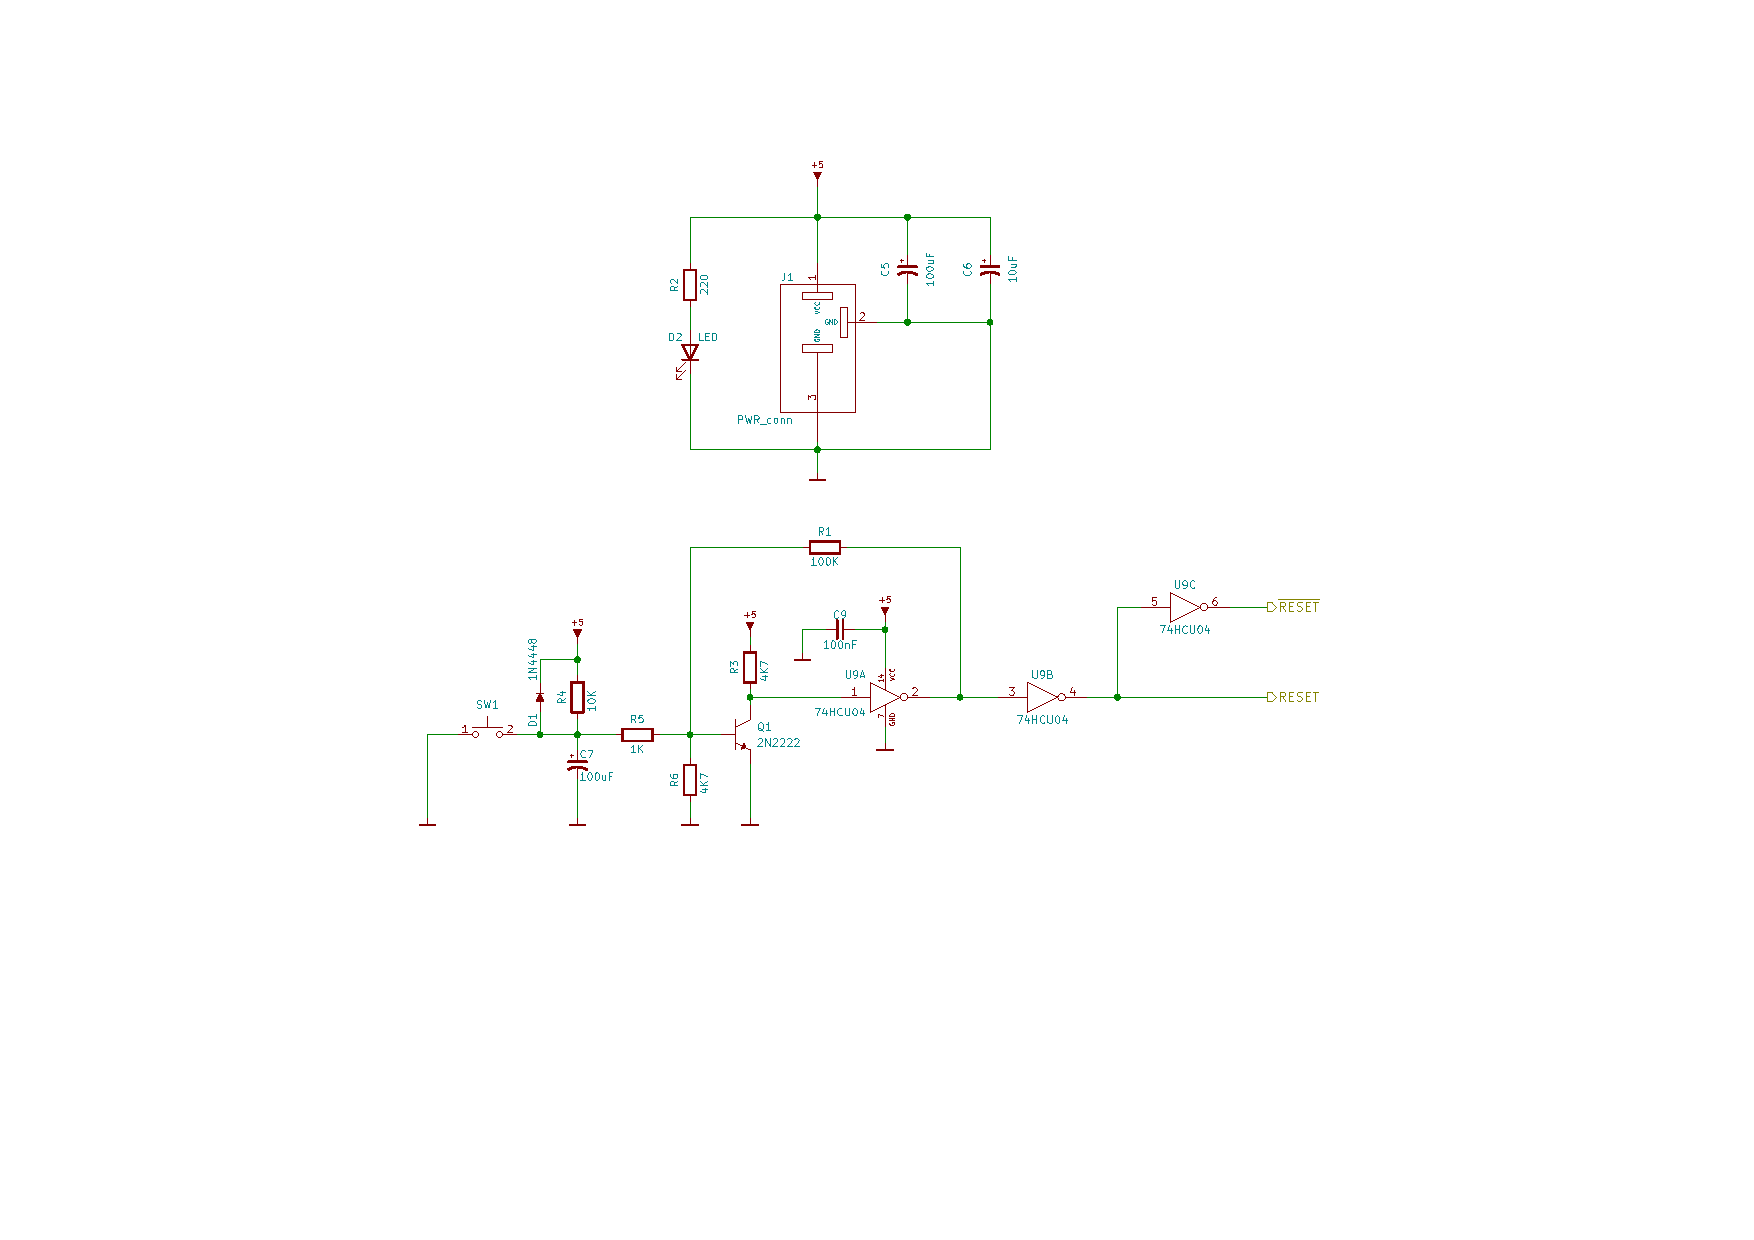
\includegraphics[width=0.5\linewidth,trim={11cm 12.8cm 12.4cm 2.5cm},clip]{figures/artemisa-schematic-power}
  \caption{Schematic diagram of power connector}
  \label{fig:artemisa-schematic-power-conn}
\end{figure}

The LED \toref{diode} {\tt D2} is used to indicate the computer is powered on when the power cable is connected to {\tt J1}. The resistor {\tt R2} is used to limit the current passing throught {\tt D2}.

\begin{theory}[h]{Diodes}
  Diodes are semiconductor devices that conduct the electric current only in one direction. They have two terminals: the anode and the cathode. The current flows from the anode to the cathode (forward current), but never from the cathode to the anode (reverse current). The forward current experiments a voltage drop of a few volts caused by the junction of semiconductor material in the diode, typically of 0.6-0.7 volts.\\\\

  LEDs, or light-emitting diodes, are a special kind of diodes that emits light when forward current flows through it. Their voltage drop depends on the color of the light they emit, and it is typically of a few volts. Apart from this particularity, their behavior is the same as any other type of diode.\\\\

  Any diode, LEDs included, does not offer any resistance to the forward current. The current experiments a voltage drop as discussed above. But once that voltage drop is exceeded, all the current will flow following the Ohms law. This means that, in the absence of any other kind of resistor in the circuit, the current will be theorically infinite (as $I = \frac{V}{R}\), when $R\) is zero). Or, in other words, a short-circuit will happen.\\\\

  For that reason, LEDs are always put in series with a resistor that will limit the current that traverses the circuit. Otherwise, we will have a short-circuit that will destroy the LED, and could damage the power supply.
\end{theory}

You can also find two large electrolytic capacitors: {\tt C5} and {\tt C6}. They are \toref{decoupling capacitors} used to filter the voltage fluctuations that may occur in the power adapter connected to {\tt J1}.

\begin{theory}[h]{Decoupling capacitors}
  Integrated circuits do not consume an even electric current. They experiment fluctuations. They work like a building. If many occupiers open their water taps, the whole building will demand a high flow of water from the external water supply. If most of them close their taps, the flow will be low. Integrated circuits are made of transistors. And each transistor is equivalent to a water tap. They are open or closed depending on their inputs and their previous states.\\\\

  When part of the circuit experiments a spike in their current demand, the power supply must satisfy it. However, power supplies are not ideal. They will try to adequate the supplied voltage to the new demands. But it does not happen immediately. As result, some parts of the circuit could experiment a brief voltage drop. This can have effects to the integrated circuits, generating errors like misinterpreting digital input values.\\\\

  The way to prevent this is to use decoupling capacitors. They will act as local batteries connected to some part of the circuit. If there is any voltage drop in the power input, the charge of the capacitor will compensate the lost. The capacitor will operate as a power supply for a short period of time (while it is charged), ensuring the voltage level is even regardless the fluctuations in the supply and the demand. In the building analogy, this is like putting a water tank at the input pipe of the building. All occupiers can open their taps all at once. The tank will feed the taps while the water supplier adapts the flow to the new demand.\\\\

  Typically, every integrated circuit has its own small decoupling capacitor to protect it from the voltage fluctuations. There are also some bulk capacitors aimed to decouple the whole power circuit of the board from the power line coming from the DC barrel connector.
\end{theory}

The second part of the schematic sheet shown in figure \ref{fig:artemisa-schematic-por} is the power-on reset circuit. This part is by far more complex than the other. And also more complex than most of the circuits we will analyze in this book. So we will explain how it works with an analysis of how the current flows on power on and how it affects the \sym{RESET} and \sym{/RESET} outputs.

\begin{figure}[h]
  \centering
  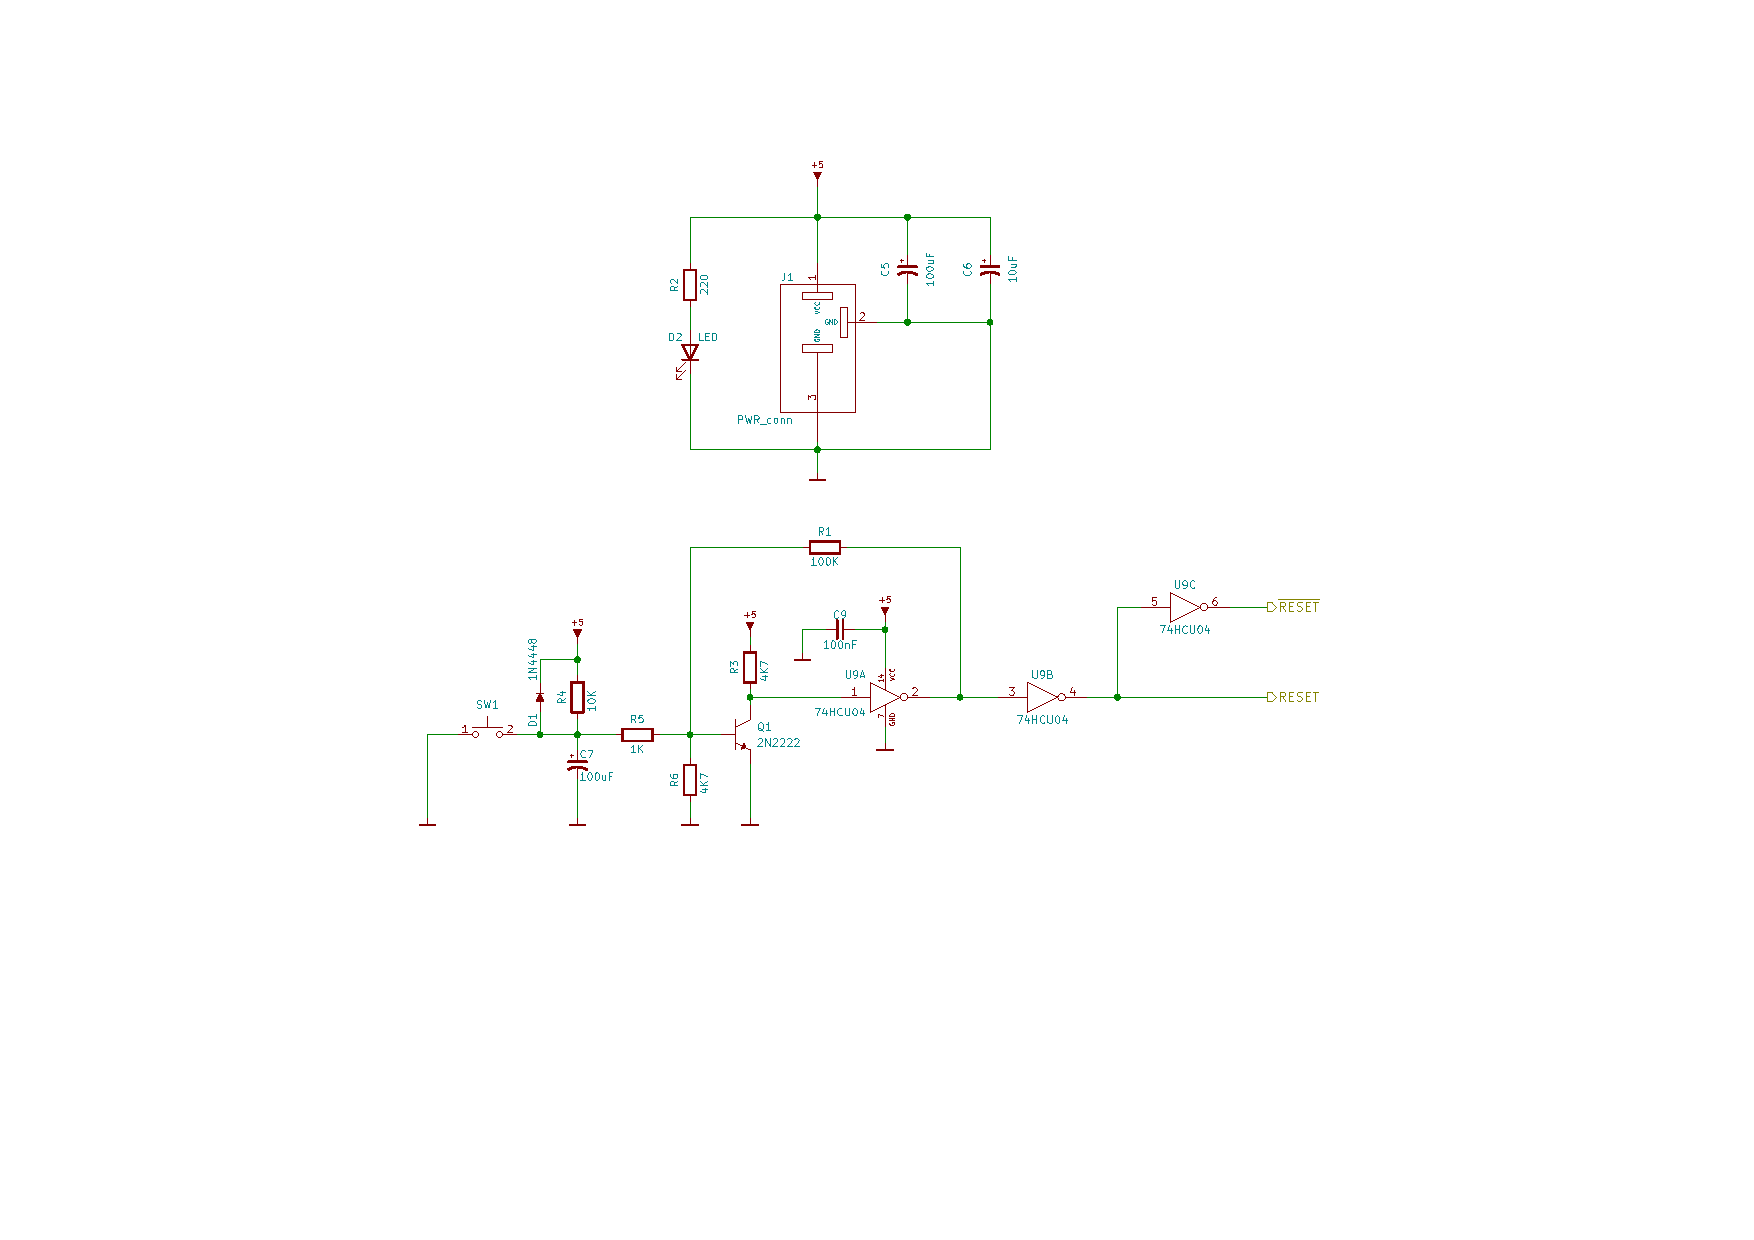
\includegraphics[width=\linewidth,trim={6cm 7cm 6cm 8.5cm},clip]{figures/artemisa-schematic-power}
  \caption{Schematic diagram of power-on reset circuit}
  \label{fig:artemisa-schematic-por}
\end{figure}

We will start assuming we just have connected the power cable to the DC barrel connector. At that instant, the current is ready to flow from the {\tt +5} power supply throught {\tt R4} to reach the positive terminal of the capacitor {\tt C7}. We will assume this capacitor is discharged because the circuit was not energized yet. So the voltage in its positive terminal is initially zero. This also means there is almost no current through {\tt R5} or {\tt R6}.

\begin{theory}[h]{Transistors}
  Transistors are semiconductor devices used to amplify or switch electronic signals. They have three terminals. The voltage level between a pair of these terminals determine the current through another pair of terminals. The power of the controlled output can be higher than the power of the controller input. Thus, they can amplify a electric signal.\\\\

  In this particular example of figure \ref{fig:artemisa-schematic-por}, we are using a NPN bipolar transistor for switching purposes. These transistors have three terminals known as base (left), emitter (below, with an arrow) and collector (above). The current between base and emitter ($I_B$) determines the current that will go from the collector to the emitter ($I_C$).

  \begin{itemize}
    \item When the voltage at the base terminal is low, there will be no current from the base to the emitter. Thus, the transistor will be cut-off and no current will flow. The collector-emitter junction will be equivalent to an open circuit.
    \item If the voltage at the base terminal is high, the transistor will saturate and will let pass as much current as possible from the collector to the emitter. The collector-emitter junction will be equivalent to a closed circuit.
  \end{itemize}

\end{theory}

Now its time to analyze the \toref{transistor} {\tt Q1}. This is used as a switching transistor. As the base current $I_B$ is zero, the transistor is cut-off. This makes the collector-emitter junction to be equivalent to an open circuit. Thus, the 5 volts across {\tt R3} are \toref{transmitted to the input terminal} of the 74HCU04 logic inverter {\tt U9A}.

\begin{theory}[h]{Voltage drop when current is zero}
  Perhaps you might wonder why the input terminal of {\tt U9A} has 5 volts when {\tt Q1} is cut-off considering there is a resistor {\tt R3} in the path. The aswer to this is given by the Ohms law.\\\\

  As {\tt Q1} is cut-off, there is only one possible path for the current: from {\tt 5+} to the input terminal of the logic inverter {\tt U9A}. The logic inverter, as any other logic gate, has a huge input impedance around 6M\si{\ohm}. This means the current going through the logic gate input terminal is almost zero. The voltage in the input terminal of {\tt U9A} is the five volts from the power supply minus the voltage drop in {\tt R3}, or $V_{in} = 5v - V_{R3}$. If there is no current, the Ohms law $V=I \cdot R$ reveals the voltage drop $V_{R3}$ is zero. Thus, the voltage at the input terminal of the logic gate is 5 volts.\\\\

  The rule of thumb is that, in the absence of current due to very high impedances, the voltage remains constant in all those points where current is not flowing. No matter the resistors we put on its way.
\end{theory}

As the logic inverter {\tt U9A} receives 5v in its input, or a high level in the digital world, it generates 0v in the output, a low level. The inverter {\tt U9B} inverts the value again, so {\tt RESET} signal is high. {\tt U9C} inverts that signal one more time to generate {\tt /RESET}, which will be low. In other words, this is the activation of our reset pulses immediately after the power connector is plugged.

Now let us come back to the capacitor {\tt C7}. As we said before, the current from the power supply is flowing through {\tt R4} to the input terminal of the capacitor. This will initiate the charging cycle of the capacitor, what requires some time to complete. During that time, it will be draining the current coming from the power supply throught {\tt R4}. And the voltage in its positive terminal will increase slowly, following a loading curve similar to the one shown in figure \ref{fig:cap-curves}.

\begin{figure}[h]
  \centering
  \includegraphics[width=0.7\linewidth,trim={1cm 3cm 1cm 3cm},clip]{figures/cap-charge-curve}
  \caption{Charging curve of a capacitor}
  \label{fig:cap-curves}
\end{figure}

As the time passes, the capacitor will increase its charge and voltage. And that will also increase the current going through {\tt R5} and {\tt R6}. Part of this current will go through the base terminal of the transistor {\tt Q1}, making it leave the cut-off region to enter the active region. When this happens, the collector-emitter current will be the base current amplified by the transistor gain: $I_C = h_{FE} \cdot I_B$. This will cause a voltage drop in {\tt R3} due to that current, with an interesting side effect: the voltage at the input terminal of {\tt U9A} will be reduced.

So in summary, the voltage of the input terminal of {\tt U9A} is inversely proportional to the charge of the capacitor {\tt C7}. The more charge in the capacitor, the less voltage in the logic inverter. Approximately 100ms after power on, the voltage in the input of {\tt U9A} will reach a point that will make its output to transit from low to high. The rest of inverters {\tt U9B} and {\tt U9C} will change their state as well. So the level of {\tt RESET} will pass to be low and the level of {\tt /RESET} will pass to be high. That is the effective termination of the reset pulse.

Now we can put all out attention in the resistor {\tt R1}. This is a positive feedback circuit that connects the output of {\tt U9A} to the base terminal of {\tt Q1}. While this transistor is in the cut-off region, the output of {\tt U9A} has zero volts. Not making any significant effect in the circuit. When the transistor enters the active region and the state of {\tt U9A} transits, the output of this inverter will have 5 volts. This will drive a current that will go through {\tt R1} to join and increment $I_B$ in {\tt Q1}. This increment in $I_B$ will increase $I_C$, making the transistor to reach the saturation region much faster. In other words, the feedback resistor {\tt R1} is giving a push to the speed at which $I_B$ and $I_C$ increases. This is particularly useful to ensure the rising edge of {\tt U9A} (and the rest of inverters) is as vertical and fast as possible, as we will discuss soon.

If you pay attention, you will see the logic inverter {\tt U9A} is {\tt 74HCU04} instead of {\tt 74HC04}. That extra {\it U} means {\it unbuffered}. One of the multiple particularities of unbuffered gates is that they have very low output oscillations when the inputs are slow. An 74HC04 part here could cause output oscillations while the input signal is around the logic level threshold. If the input voltage decreases too slowly around that point, the buffered gate would respond with a quick transition, and any noise in the line could make it to transit back again, generating an undesired oscillation as shown in Figure \ref{fig:oscilloscope-slow-input}.

\begin{figure}[h]
  \centering
  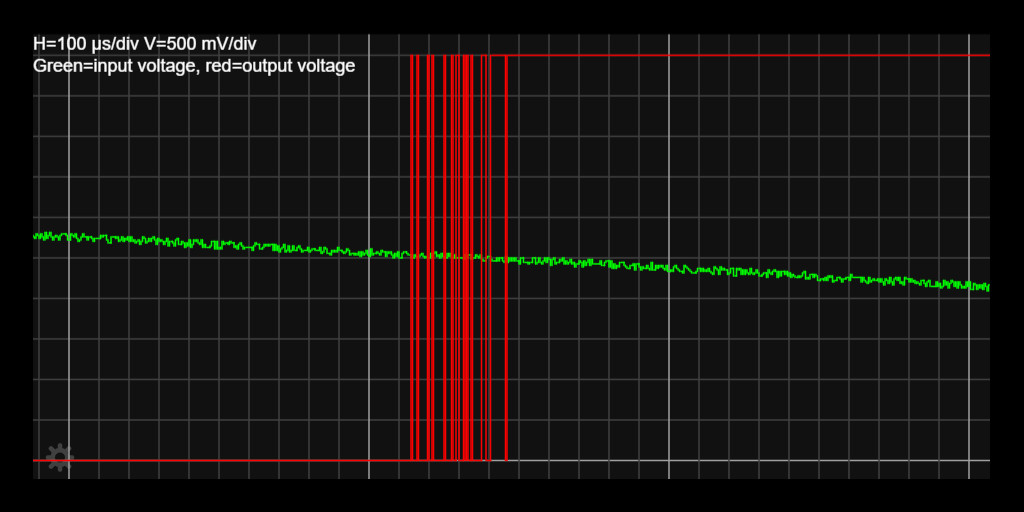
\includegraphics[width=1\linewidth]{figures/oscilloscope-slow-input}
  \caption{Output oscillation in a logic inverter caused by noise in a slow input}
  \label{fig:oscilloscope-slow-input}
\end{figure}

The output oscillation in {\tt U9A} would be detected by devices connected to {\tt RESET} and {\tt /RESET} as a sequence of false reset pulses. What is a huge problem considering that many devices require the reset pulse to last for several milliseconds. The fast oscillations will leave them in a inconsistent state that will derive in a erratic behaviour.

This is an actual problem in this design, because the input of {\tt U9A} is connected to the output of the transistor {\tt Q1}, which will ramp down its voltage as the capacitor {\tt C7} is charged. This is a clear case of slow signal that will take some milliseconds to transit from the high to the low logic state.

The circuits uses two elements to prevent the slow output problem. One is the usage of the positive feedback added to the transistor {\tt Q1} discussed above. Thanks to this, the $I_B$ of the transistor is incremented once the output of {\tt U9A} transists from low to high. What pulls the voltage down at the input of {\tt U9A}, making it leave the transistion level threshold very quickly. The second element is the usage of an unbuffered logic inverter instead of a buffered one. Buffered gates have a high linear-mode gain that can lead to oscillations with a low noise in the input. In contrast, unbuffered gates do not tend to oscillate unless the noise is much bigger.

Finally, at the left side of the circuit you can see a switch {\tt SW1} and a diode {\tt D1}. The diode is used to discharge the capacitor {\tt C7} quickly when the power is disconnected. When that happens, the {\tt 5+} power will not drive 5 volts any longer, and it can drain the charge of the capacitor going through {\tt D1}. The switch {\tt SW1} is used to force a reset signal in the circuit. It will connect the positive terminal of the capacitor {\tt C7} to the ground. In both cases, when power is switched off or the reset button is pressed, the capacitor {\tt C7} is discharged and it reaches a voltage close to zero. This will cause the same interactions in {\tt Q1} and {\tt U9A} we have seen above, initiating a new reset pulse that will last around hundred milliseconds.
